\documentclass[a4paper,17pt]{extarticle}
\usepackage[utf8]{inputenc}
\usepackage{amsmath}
\usepackage{amssymb}
\usepackage{fontspec}
\usepackage[T1]{fontenc}
\usepackage{caption}
\usepackage{hyperref}
\usepackage{array}
\usepackage{tabularx}
\usepackage{graphicx}
\usepackage{background} 
\backgroundsetup{contents=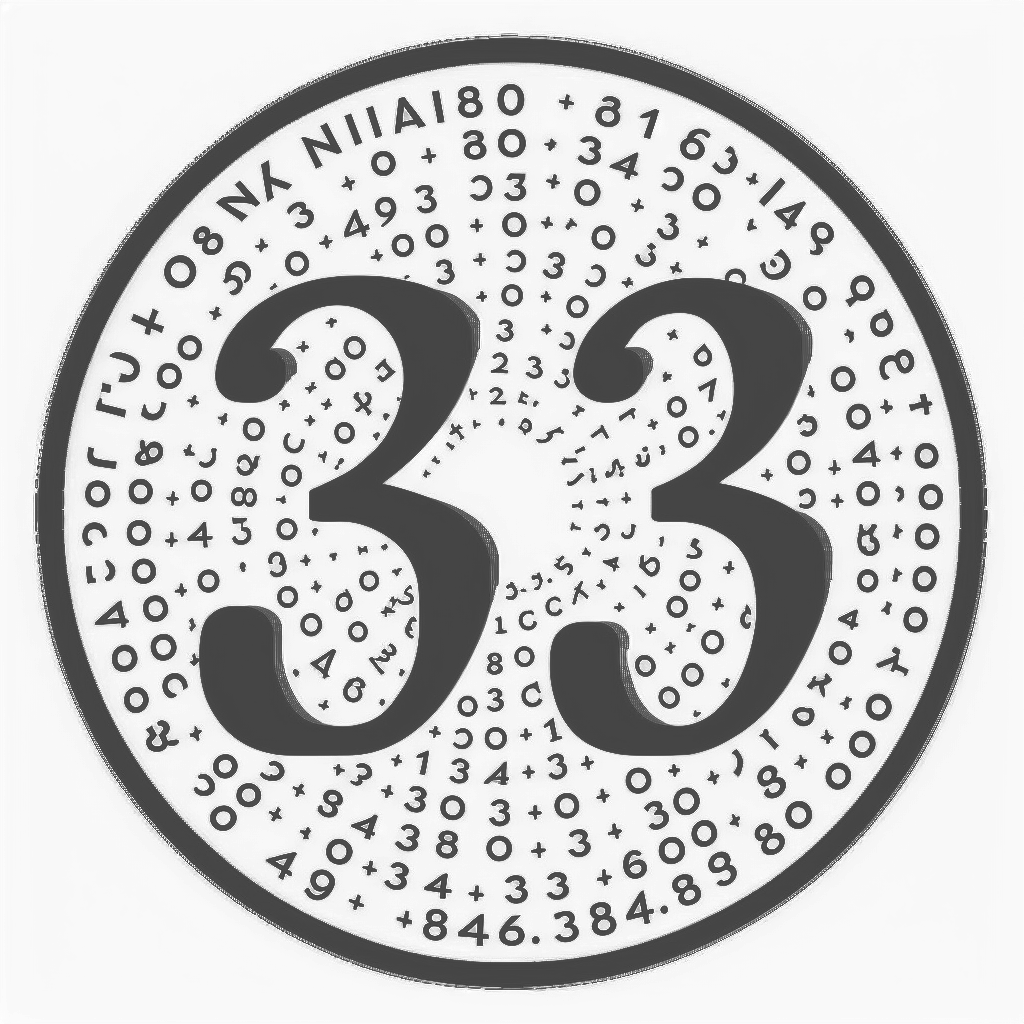
\includegraphics{static/logo.png}, opacity=0.1, scale=.3, angle=0}
\title{\LARGE \textsf{{Optional Mathematics - SEE Model Solutions}}}
\author{\textsf{Saugat Dhakal, Asal KC}}
\date{\textsf{28th Janurary, 2023}}
\begin{document}
\setsansfont{DMSans}[
    Path=./static/,
    Scale=0.9,
    Extension = .ttf,
    UprightFont=*-Regular
    ]
\maketitle
\section{\textsf{Model Set 1}}
\textsf{1. a) What is a trigonometric function? \\ 
 - A trigonometric function is a special type of function which
 contains trigonometric ratios and an angle. 
For example, sinx, cosx etc.
\\ \\
1. b) What is the arithmetic mean between two numbers a and b? \\
 - The arithmetic mean between two number a and b is $\frac{a + b}{2}$. \\ \\
2. a) Write a set of numbers which is continuous on a number line? \\
 - The set of real numbers is continuous on a number line. \\ \\
2. b) If matrix A = \begin{bmatrix}
p & q \\
r & s 
\end{bmatrix}, what is the value of |A|? \\
 - The value of |A| = ps - qr. \\ \\
 3. a) If the slopes of two straight lines are $m_1$ and $m_2$ respectively and $\theta$ be the angle between them, write the formula for tan$\theta$. \\
 - The formula of tan$\theta$ is given by, tan$\theta$ = $\frac{m_1 - m_2}{1 + m_1m_2}$. \\ \\
 3. b) Which geometric figure will be formed if a plane intersects a cone parallel to its base? \\
 - A circle will be formed if a plane intersects a cone parallel to its base. \\ \\
 4. a) Express sin2A in terms of tanA. \\
 - sin2A in terms of tanA is given by, sin2A = $\frac{2tanA}{1 + tan^2A}$. \\ \\
 4. b) Define angle of elevation. \\
 - An angle of elevation is defined as an angle between the horizontal plane and line of sight from the observer's eye to some object above. \\ \\
 5. a) What is the scalar product between two vectors $\overrightarrow{a}$ and $\overrightarrow{b}$ if the angle between them is $\theta$? \\
 - The scalar product between two vectors $\overrightarrow{a}$ and $\overrightarrow{b}$ if the angle between them is $\theta$ is |a||b|cos$\theta$. \\ \\
 5. b) In an inversion transformation if P' is the image of P and r is the radius of inversion circle with centre O, write the relation of OP, OP' and r. \\ 
 - The relation between OP, OP' and r is given by $r^2$ = OP.OP'. \\ \\
 6. a) Find the inverse of f(x) = 4x + 5. \\
 - Solution, \\
 Let, y = f(x) = 4x + 5, \\
 Since, y = f(x), then $f^{-1}$(y) = x, \\
 then y = 4x + 5 \\
 or, y - 5 = 4x \\
 or, x = $\frac{y - 5}{4}$ \\
 or, $f^{-1}$(y) = $\frac{y - 5}{4}$ \\
 or, $f^{-1}$(x) = $\frac{x - 5}{4}$ \\
 Therefore, the inverse of the given function is $\frac{x - 5}{4}$. \\ \\
 6. b) If g(x) = 2x - 1 and f(x) = 4x, find the value of gof(x). \\
 - Given, g(x) = 2x - 1 and f(x) = 4x \\
 gof(x) = g[f(x)] = g(4x) = 2(4x) - 1 = 8x - 1 \\
 Therefore, gof(x) = 8x - 1. \\ \\
 7. a) If A = $\begin{bmatrix}
     2 & -1 \\
     3 &  1
 \end{bmatrix}$, find |A| and write if the inverse of A is defined or not. \\
 - Given, A = $\begin{bmatrix}
     2 & -1 \\
     3 &  1
 \end{bmatrix}$ \\
 So, |A|  = 2(1) - (-1)(3) = 2 + 3 = 5 \\
 Since |A| is not equal to zero, the inverse of the matrix exists. \\ \\ 
 7. b) According to Cramer's Rule, find the values of $D_1$ and $D_2$ for ax + by = c and px + qy = r. \\ 
 - We know, $D_1 = \begin{vmatrix}
     c & b \\
     r & q
 \end{vmatrix}$ = cq - br and 
 $D_2 = \begin{vmatrix}
     a & c \\
     p & r
 \end{vmatrix}$ = ar - pc \\ \\
 8. a) Find the slopes of two straight lines 3x + 4y + 5 = 0 and 6x + 8y + 7 = 0 and write the relationship between them. \\
 - The given lines are 3x + 4y + 5 = 0 and 6x + 8y + 7 = 0, \\
 then, $m_1$ = $\frac{-a}{b} = \frac{-3}{4}$ \\
 and, $m_2$ = $\frac{-a}{b}$ = $\frac{-6}{8}$ = $\frac{-3}{4}$ \\
 The relation between the slopes is that they are equal. \\ \\
 8. b) Find the single equation for the pair of lines represented by 3x + 2y = 0 and 2x - 3y = 0. \\
 - The single equation for the following pair of lines is represented by, \\
 (3x + 2y)(2x - 3y) = 0 \\
 6$x^2$ - 9xy + 4xy - 6$y^2$ = 0\\
  6$x^2$ - 5xy - 6$y^2$ = 0\\
  The required equation is 6$x^2$ - 5xy - 6$y^2$ = 0. \\ \\
9. a) Convert sin6A.cos4A into sum or difference of sine or cosine. \\
- sin6Acos4A \\ = $\frac{1}{2}$(2sin6A.cos4A) \\ = $\frac{1}{2}$(sin(6A + 4A) + sin(6A - 4A)) \\ = $\frac{1}{2}$(sin(10A) + sin(2A)) \\ \\
9. b) If 2sin2$\theta$ = $\sqrt{3}$ find the value of $\theta$ (0 $\leq$ $\theta$ $\leq$ 180). \\
- Given, 2sin2$\theta$ = $\sqrt{3}$ \\
or, sin2$\theta$ = $\frac{\sqrt{3}}{2}$ \\
or, 2$\theta$ = 60, 120 \\
or, $\theta$ = 30, 60. \\
Therefore, the required values are 30 and 60. \\ \\
10. a) Find the angle between two vectors $\overrightarrow{a}$ and $\overrightarrow{b}$ if |$\overrightarrow{a}$| = 2, |$\overrightarrow{b}$| = 12 and $\overrightarrow{a}.\overrightarrow{b}$ = 12. \\
Solution, \\
Let, $\theta$ be the angles between the two vectors, then, \\
cos$\theta$ = $\frac{\overrightarrow{a}.\overrightarrow{b}}{|\overrightarrow{a}||\overrightarrow{b}|}$ \\ 
cos$\theta$ = $\frac{12}{2.12}$ \\ 
cos$\theta$ = $\frac{1}{2}$ \\ 
cos$\theta$ = cos60  \\
$\theta$ = 60\\
Therefore, the angle between the two vectors is 60. \\ \\
\begin{figure}[htp]
    \centering
    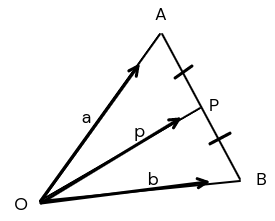
\includegraphics[width=6cm]{static/Screenshot from 2023-01-28 15-30-36.png}
    \caption{10. b)}
    \label{fig:question}
\end{figure}
10. b) From the given figure, find $\overrightarrow{AP}$ and express $\overrightarrow{p}$ in terms of $\overrightarrow{a}$ and $\overrightarrow{b}$. 
Solution, \\
From the figure, $\overrightarrow{OA}$ + $\overrightarrow{AP}$ = $\overrightarrow{OP}$ \\
then, $\overrightarrow{AP}$ = $\overrightarrow{OP}$ - $\overrightarrow{OA}$ \\
or, $\overrightarrow{AP}$ = $\overrightarrow{p}$ - $\overrightarrow{a}$ ... (1) \\
Similarly, \\
$\overrightarrow{BP}$ = $\overrightarrow{p}$ - $\overrightarrow{b}$ ... (2) \\ 
Adding (1) and (2), we obtain, \\
2$\overrightarrow{p} = $\overrightarrow{a} + $\overrightarrow{b}$ ($\overrightarrow{BP}$ + $\overrightarrow{AP}$ = 0) \\
$\overrightarrow{p} = \frac{1}{2}$(\overrightarrow{a} + $\overrightarrow{b}$) 
which is the required value of the vector. \\ \\ 
11. Solve: $x^3 - 3x^2 - 4x + 12 = 0$. \\ 
Solution, \\
The given equation is $x^3 - 3x^2 - 4x + 12 = 0$, the constant term in this equation is 12. The factors of 12 are $\pm1$, $\pm2$, $\pm3$, $\pm4$, $\pm6$ and $\pm12$. \\ 
Let, f(x) = $x^3 - 3x^2 - 4x + 12$, then \\
f(1) = 1 - 3 - 4 + 12 = 6 \\
f(-1) = -1 - 3 + 4 + 12 = 12 \\
f(2) = 8 - 12 - 8 + 12 = 0 \\
So, (x - 2) is a factor of f(x) \\
then, \\
$x^3 - 3x^2 - 4x + 12 = 0$ \\ 
or, $x^3 - 2x^2 - x^2 + 2x - 6x + 12 = 0$ \\
or, $x^2(x - 2) - x(x - 2) - 6(x - 2)= 0$ \\
or, $(x - 2)(x^2 - x- 6) = 0$ \\
or, $(x - 2)(x^2 + 2x - 3x- 6) = 0$ \\
or, $(x - 2)(x + 2)(x - 3) = 0$ \\
then, we get, x = 2, x= -2 and x = 3. \\
The required values are 2, -2 and 3. \\ \\
12. Optimize P = 5x + 4y under the given constraints: x - 2y $\leq$ 1, x + y $\leq$ 4, x $\geq$ 0 and y $\geq$ 0. \\
Solution, the given inequalities are x - 2y $\leq$ 1, x + y $\leq$ 4, x $\geq$ 0 and y $\geq$ 0, \\
Converting inequalities to equations, we get, \\
x - 2y = 1 ... (1) \\
x + y = 4 ... (2) \\
x = 0 ... (3) \\
y = 0  ... (4) \\
In equation 1, we have (x,y) = (1,0) and (3,1) as two solutions. Let, (0,0) be a test point. Then, x - 2y $\leq$ 1 becomes 0 $\leq$ 1 which is true. Therefore, the inequality contains origin as well. \\
In equation 1, we have (x,y) = (0,4) and (4,0) as two solutions. Let, (0,0) be a test point. Then, x + y $\leq$ 4 becomes 0 $\leq$ 4 which is true. Therefore, the inequality contains origin as well. \\
The feasible region contains the vertices (0,0), (1,0), (3,1) and (0,4). \\ \\
\begin{tabularx}{1\textwidth} { 
  | >{\raggedright\arraybackslash}X 
  | >{\centering\arraybackslash}X 
  | >{\raggedleft\arraybackslash}X | }
 \hline
 Vertices & P = 5X + 4Y & Remarks \\
 \hline
 (0,0) & 0 & Minimum \\
 \hline
 (1,0) & 5  &   \\
\hline
 (3,1)  & 19  & Maximum  \\
\hline 
(0,4)  & 16  &  \\
\hline
\end{tabularx} \\
Therefore, the minimum value is 0 at (0,0).
13. For a real valued function f(x) = 2x + 3. \\
a) Find f(2.95), f(2.99), f(3.01), f(3.05) and f(3). \\
Solution, \\
f(2.95)  = 2(2.95) + 3 = 8.9 \\
f(2.99)  = 2(2.99) + 3 = 8.98 \\
f(3.01)  = 2(3.01) + 3 = 9.02 \\
f(3.05)  = 2(3.05) + 3 = 8.10 \\
f(3)  = 2(3) + 3 = 9 \\
b) Is this function continous at x = 3? \\
\[ \lim_{x\to3^+} f(x) 	= 2(3) + 3 = 9  \]\\ 
\[ \lim_{x\to3^-} f(x) 	= 2(3) + 3 = 9 \]\\ 
\[f(3) = 9\] \\
Since, the left hand limit, right hand limit and the functional value are equal, the function is continuous at x = 3. \\ \\
14. By using matrix method, solve the following system of equations: 3x + 5y = 11, 2x - 3y = 1. \\
Solution, the given equations are 
\[3x + 5y = 11 ... (1)\] 
\[2x - 3y = 1 ... (2)\] 
Converting the given equations to matrices, we get, \\ \\
\begin{bmatrix}
    3 & 5 \\
    2 & -3
\end{bmatrix}
\begin{bmatrix}
    x \\
    y
\end{bmatrix} = 
\begin{bmatrix}
    11 \\
    1
\end{bmatrix} 
which is in the form of AX = B. \\
then, X = A$^{-1}$B. \\
For inverse of A, |A| = -19 and adjoint = \begin{bmatrix}
    -3 & -5 \\
    -2 & 3
\end{bmatrix} \\ 
So, \begin{bmatrix}
    x \\
    y
\end{bmatrix} = 
$\frac{1}{-19}$\begin{bmatrix}
    -3 & -5 \\
    -2 & 3
\end{bmatrix} 
\begin{bmatrix}
    11 \\
    1
\end{bmatrix} \\
On multiplying and solving, we get, x = 2 and y = 1. \\ \\
15. Find the single equation of pair of straight lines passing through the origin and perpendicular to the lines represented by $2x^2 - 5xy + 2y^2 = 0$. \\
Solution, the given equation is $2x^2 - 5xy + 2y^2 = 0$, after factorization we get, $(x - 2y)(2x - y) = 0$, \\
So, the required lines are \\
x - 2y = 0 ... (1) \\
2x - y = 0 ... (2) \\
The equation of line perpendicular to (1) and passing through the origin is given by 2x + y = 0 ... (3) \\
The equation of line perpendicular to (2) and passing through the origin is given by x + 2y = 0 ... (4) \\
Combining, (3) and (4), we obtain $2x^2 + 5xy + 2y^2 = 0$, which is the required equation. \\ \\
16. Find the value of: \\ \\
$sin(20).sin(30).sin(40).sin(80)$ \\
= $\frac{1}{2}sin(20).sin(40).sin(80)$ \\
= $\frac{1}{4}(2sin(20).sin(40)).sin(80)$ \\
= $\frac{1}{4}(cos(20) - cos(60)).sin(80)$ \\
= $\frac{1}{4}(cos(20) - \frac{1}{2}).sin(80)$ \\
= $\frac{1}{4}$$\frac{(2cos(20).sin(80) - sin(80))}{2}$ \\
= $\frac{2cos(20)cos(10) - cos(10)}{8}$ \\
= $\frac{cos(30) + cos(10) - cos(10)}{8}$ \\
= $\frac{\sqrt{3}}{16}$
\\ \\
17. If A + B + C = $\pi$, prove that:
\[sin^2A - sin^2B + sin^2C = 2sinAcosBsinC\] \\
Solution, \\
A + B + C = $\pi$ => sin(A + B) = sinC and cos(A + B) = -cosC \\ 
then, 
LHS = $sin^2A - sin^2B + sin^2C$ \\ 
= $sin^2A - sin^2B + sin^2C$ \\ 
= $\frac{1}{2}(1 - cos2A) - \frac{1}{2}(1 - cos2B) + sin^2C$ \\
= $\frac{1}{2}(cos2B - cos2A) + sin^2C$ \\ 
= $\frac{1}{2}(2sin(A + B)sin(A - B)) + sin^2C$ \\
= $sinCsin(A - B) + sinC.sin(A + B)$ \\
= $sinC(sin(A - B) + sin(A + B))$ \\
= $2sinAcosBsinC$ \\
= RHS \\ 
Therefore, LHS = RHS proved. \\ \\}
\end{document}
